 \documentclass{report}
 
\usepackage[utf8]{inputenc} 
\usepackage[T1]{fontenc}      
\usepackage[top=2.0cm, bottom=3cm, left=3.0cm, right=3.0cm]{geometry}
\usepackage{graphicx}
\usepackage{amsmath}
\graphicspath{{figures/}{../figures}}

\begin{document}

\section*{Exercice 1 $\bullet\bullet\circ$}

Le cadre en pointillé représente un quadripôle tel que : $u_{s}=Gu_{e}$.

\begin{figure}[!h]
\centering
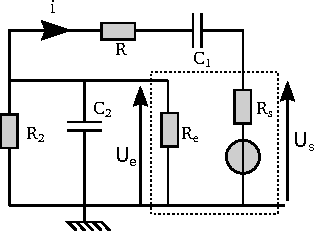
\includegraphics[width=0.5\linewidth]{circuit_5.pdf}
\end{figure}

\begin{itemize}

\item[•] On suppose d'abord que $R_{s}=0$ et $R_{e}=\infty$. Trouvez  une équation différentielle en $i(t)$. Quelle est la condition sur $G$ pour voir apparaître des oscillations ? Donnez alors la valeur $f_0$ des oscillations.

\item[•] Comment cette condition change lorsque $R_{s}\neq 0$ et $R_{e}\neq\infty$?

\end{itemize}

\newpage

\section*{\textit{Correction Exercice 1}}

\begin{itemize}
	\item[•] Pour ne pas se faire déstabiliser, on peut raisonner sur le filtre constitué du circuit en dehors de la zone en pointillé : Il s'agit d'un filtre classique dont la fonction de transfert est facile à trouver. L'intensité $I$ étant proportionnelle à la tension $u_e$, on tombe facilement sur la même équation différentielle :
	\begin{equation}
		i(t) + \left[(1-G)R_2C_1 +R_1C_1+R_2C_2\right]\frac{di(t)}{dt}+R_1C_1R_2C_2\frac{d^2i(t)}{dt^2}=0 
	\end{equation}
	\item[•]  $G=\frac{R_1C_1+R_2C_2+R_2C_1}{R_2C_1}$ et $f_0=\frac{1}{2\pi(R_1C_1R_2C_2)}$
	\item[•] On remplace $R_2\leftarrow\frac{R_2R_e}{R_2+R_e}$ et $R_1\leftarrow R_1+R_s$
\end{itemize}

\newpage

\section*{Multivibrateur astable $\bullet\bullet\circ$}

On considère le montage suivant.

\begin{figure}[!h]
\centering
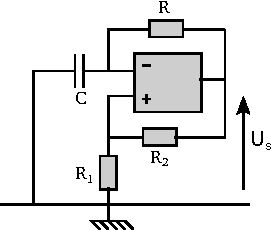
\includegraphics[width=0.45\linewidth]{circuit_3.pdf}
\end{figure}

\subsubsection{Amplificateur idéal}

On suppose l'AO idéal : rappeler ses caractéristiques. Dans la suite, on notera $\tau_1=RC$.

\begin{itemize}
	\item[$\clubsuit$] Comment se comporte t-il dans cette situation ? Pourquoi ?
	
	\item[$\clubsuit$] Etablir l'équation différentielle vérifiée par $u_-(t)$.

	\item[$\clubsuit$] Déterminer l'évolution temporelle de  $u_{-}(t)$ et $u_{s}(t)$. On pourra prendre pour condition initiale $u_-(t=0)=R_1/(R_1+R_2)\times V_{sat}$.
\end{itemize}

\subsubsection{Amplificateur réel}

On considère désormais que l'amplificateur est réel, c'est-à-dire que les tensions $u_+$, $u_-$ et $u_s$ vérifient la relation suivante : 
	\begin{equation}
		\tau_0\frac{du_s}{dt} +u_s = \mu_0(u_+-u_-)
	\end{equation}
	avec $\mu_0=10^5$ et $\frac{\mu_0}{2\pi\tau}=$1MHz.
\begin{itemize}
	\item[$\clubsuit$] Déterminez une équation différentielle sur $u_s(t)$. Commenter les solutions. 
	\item[$\clubsuit$] Si l'on considère nulles la tension de sortie ($u_s(t=0)=0$) et la tension aux bornes du condensateur  ($u_-(t=0)=0$), pourquoi se retrouve t-on rapidement dans la situation précédente, cad avec des oscillations sur $u_s(t)$ ?
\end{itemize}

\newpage

\section*{\textit{Correction Multivibrateur astable}}

\subsubsection{Amplificateur idéal}

\begin{itemize}
	\item[•] La boucle de rétroaction est sur la borne +, l'AO est en régime saturé et donc $u_s=\pm V_s$. 

	\item[•] L'AO fonctionne en régime saturé, la condition $u_+=u_-$ n'est plus vérifiée ! On a cependant les équation suivantes (loi des noeuds en $u_+$ et loi des noeuds en $u_-$) :
	
\begin{align}
	\left\lbrace
\begin{array}{cc}
	&  u_+=\frac{R_1}{R_1+R_2}u_s\\
	\\
	&RC\frac{du_-}{dt} +u_- =u_s  \\
\end{array}\right.
\end{align}	

L'AO étant en régime saturé, $u_s=\pm V_s$, la deuxième équation correspond donc à une charge et décharge du condensateur. On peut partir de la situation où le condensateur est chargé négativement (donc $u_-<0$) et $u_s=+V_s$ (cad cohérent la condition $u_-<u_+$, toutes les autres situations s'y ramènent, juste le signe peut s'inverser). 

	Plus particulièrement, on peut commencer par $u_-(t=0)=\frac{R_1}{R_2+R_1}V_s$ et $u_+(t=0)=-V_s$ et alors :
	\begin{equation}
		u_-(t)=V_s\left(1+\frac{R_1}{R_1+R_2}\right)\exp(-t/RC)-V_s 
	\end{equation}
Puis, à $t=t_1=RC\ln\left(\frac{2R_1+R_2}{R_2} \right)$ :
	\begin{equation}
		u_-(t)=-V_s\left(1+\frac{R_1}{R_1+R_2}\right)\exp(-(t-t_1)/RC)+V_s 
	\end{equation}
Et ainsi de suite. La période est donc $T = 2RC\ln\left(\frac{2R_1+R_2}{R_2} \right)$. $u_+(t)$ évolue en créneau de même période. 
\end{itemize}

\subsubsection{Amplificateur réel}

On trouve :

\begin{align*}
	\left\lbrace
\begin{array}{cc}
	& \tau_0\frac{du_s}{dt} +u_s = \mu_0(u_+-u_-) \\
	&  u_+=\frac{R_1+R_2}{R_1}\\
	&\tau_1\frac{du_-}{dt} +u_- =u_s  \\
\end{array}\right.
\end{align*}

On arrive alors sur deux équations différentielles couplées :
\begin{align*}
	\left\lbrace
\begin{array}{cc}
	& \tau_0\frac{du_s}{dt} = \mu_1u_s - \mu_0u_- \\
	&  \\
	&\tau_1\frac{du_-}{dt} = u_s - u_-  \\
\end{array}\right.
\end{align*}
avec $\mu_1=\mu_0\frac{R_1+R_2}{R_1}-1\simeq\mu_0\frac{R_1+R_2}{R_1}$.

On toruve alors une ED sur $u_s$ :
\begin{equation}
	\frac{d^2u_s}{dt^2} +\left( \frac{1}{\tau_1}-\frac{\mu_1}{\tau_0}\right) \frac{du_s}{dt} + \frac{1}{\tau_1\tau_0}\left(\mu_0-\mu_1\right)u_s=0
\end{equation}
Comme $\mu_0<\mu_1$, les solutions sont exponentielles et divergentes. On se retrouve donc très rapidement dans le régime d'instabilité même si les conditions initiales sont nulles (la moindre perturbatiosn étant amplifiée).

\newpage

\section*{Exercice 3 $\bullet\circ\circ$}

On considère le circuit ci-dessous :

\begin{figure}[!h]
\centering
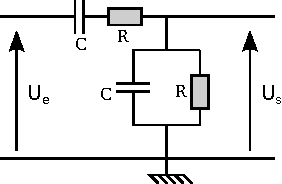
\includegraphics[width=0.5\linewidth]{circuit_1.pdf}
\end{figure}

\begin{itemize}
	\item[•] Après avoir précisé le comportement du circuit en basse et haute fréquence, déterminez la fonction de transfert de ce filtre sous la forme canonique. Quelle est l'allure de son diagramme de Bode ?
	\item[•] On réalise ce désormais le montage avec l'AO. Pour quelles valeurs de $R_1$ et $R_2$ voit-on apparaître des oscillations sur $U_{e}$?
\begin{figure}[!h]
\centering
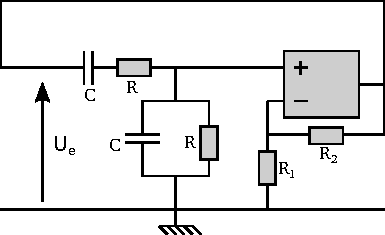
\includegraphics[width=0.6\linewidth]{circuit_4.pdf}
\end{figure}

	\item[•] Pourquoi parle t-on de régime quasi-sinusoïdal ? Décrire l'évolution du signal si les oscillations apparaissent à partir du bruit de fond électronique.
\end{itemize}

\newpage

\section*{\textit{Correction exercice 3}}

\begin{itemize}
	\item[•]
	\begin{equation}
		H=\frac{jRC\omega}{1+3jRC\omega-(RC\omega)^2}=\frac{1/3}{1+\frac{j}{3}\left( \frac{\omega}{\omega_0}-\frac{\omega_0}{\omega}\right) }
	\end{equation}
	donc $Q=1/3$ et $\omega_0=1/RC$.
	\item[•] Équation différentielle : $\omega_0\frac{du_e}{dt}=u_s+3\omega_0\frac{du_s}{dt}+\omega_0^2\frac{d^2u_s}{dt}$. Comme $u_s = (1+R_2/R_1)u_e$, on a :
	\begin{equation}
	0=u_s+\left( 2-\frac{R_2}{R_1}\right) \omega_0\frac{du_s}{dt}+\omega_0^2\frac{d^2u_s}{dt}
	\end{equation}
	Oscillations si $R_2=2R_1$.
	\item[•] Quasi-sinusoïdal car pour démarrer on a besoin de la condition $R_2>2R_1$ et alors solutions exponentielles divergentes, jusqu'à saturation. Le démarrage se fait à partir du bruit de fond qui est amplifié. 
\end{itemize}

\newpage

\section*{Exercice 4 $\bullet\bullet\circ$}

On considère le circuit ci-dessous :

\begin{figure}[!h]
\centering
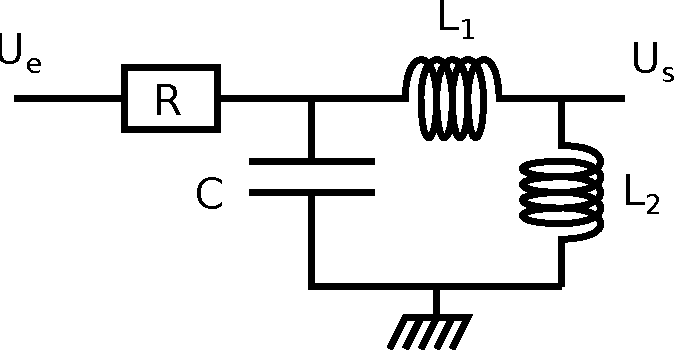
\includegraphics[width=0.4\linewidth]{resonnateur.pdf}
\end{figure}

\begin{itemize}
	\item[•]  Après avoir précisé le comportement du circuit en basse et haute fréquence, déterminez la fonction de transfert de ce filtre sous la forme canonique.
	\item[•] A quelle condition a t-on des oscillations sur le circuit avec le montage ci-dessous ?
	
	\begin{figure}[!h]
\centering
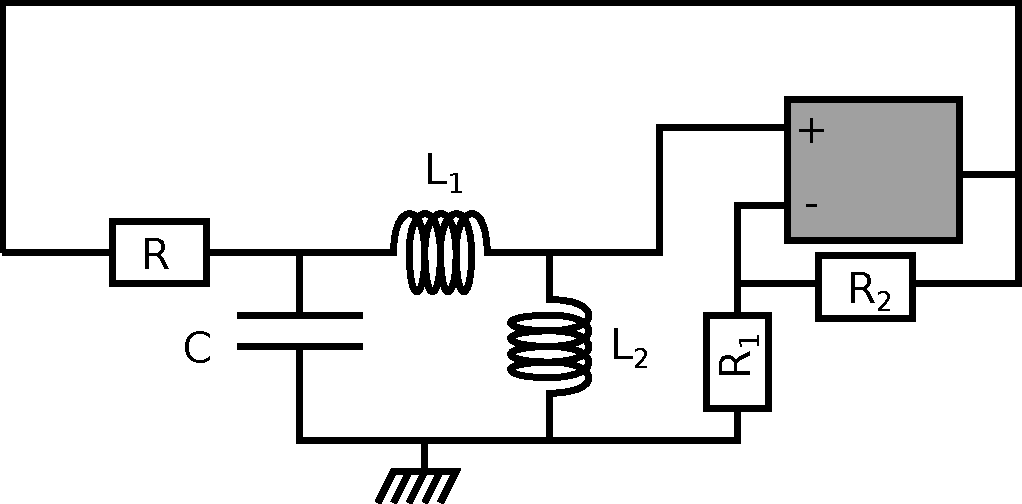
\includegraphics[width=0.4\linewidth]{resonnateur2.pdf}
\end{figure}

	\item[•] Pour éviter d'atteindre la saturation de l'AO en régime quasi-sinusoïdal, on suppose que $R_1$ est une thermorésistance, cad dont la résistance augmente proportionnellement avec la température. Expliquez comment cela permet d'éviter la saturation de l'AO.

\end{itemize}

\subsection*{Exercice supplémentaire}
Est-il possible d'avoir des oscillations sur un tel circuit si H est un passe-bas d'ordre 2 ? A quelles conditions ? 
Même questions pour un passe haut d'ordre 2.
\begin{figure}[!h]
\centering
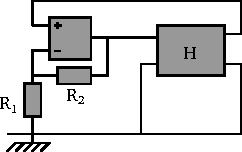
\includegraphics[width=0.3\linewidth]{circuit_9.pdf}
\end{figure}

\newpage

\section*{\textit{Correction exercice 4}}

\begin{itemize}
	\item[•] C'est un passe-bande d'ordre 2. Soit $u_1$ le potentiel entre la résistance $R$, la capacité $C$ et l'inductance $L_1$. Alors :
	\begin{equation}
		\frac{u_1}{u_e}=\frac{1}{1+R\left(\frac{1}{jL\omega}+ jC\omega \right) }
	\end{equation}
	De même :
	\begin{equation}
		\frac{u_s}{u_1}=\frac{jL_2\omega}{jL_1\omega+jL_2\omega}
	\end{equation}
	Alors : 
	\begin{equation}
		\frac{u_s}{u_e}=\frac{A_0}{1+jQ\left( \frac{\omega}{\omega_c}- \frac{\omega}{\omega_c}\right)}
	\end{equation}
	avec $\omega_c=\frac{1}{\sqrt{(L_1+L_2)C}}$, $A_0=\frac{L_2}{L_1+L_2}$ et $Q=RC\omega_c=R\sqrt{\frac{C}{L_1+L_2}}$
	
	\item[•] La fonction de transfert totale faite du filtre et de l'amplificateur d'écrit : 
		\begin{equation}
		\frac{u'_s}{u_e}=\frac{R_1+R_2}{R_1}\frac{A_0}{1+jQ\left( \frac{\omega}{\omega_0}- \frac{\omega}{\omega_0}\right)}=\frac{R_1+R_2}{R_1}\frac{A_0}{1+jR\left(C\omega- \frac{1}{L\omega}\right)}
	\end{equation}
	Le circuit est quasi-sinusoïdal s'il existe une pulsaiton $\omega_0$ tq $\mid F(j\omega_0)\mid=1$ et $arg\left[F(j\omega_0 \right] =0 $.
	
	On peut passer aussi par l'équation différentielle.
	On trouve $\omega_0=\omega_c$ et la condition :
	\begin{equation}
		\frac{R_1+R_2}{R_1}\frac{L_2}{L_1+L_2}=1
	\end{equation}
\end{itemize}

\subsubsection{Question supplémentaire}

On ne peut avoir des oscillations qu'avec un basse bande. Pour un filtre passe-haut et passe-bas, on ne peut avoir que des solutions divergentes ou qui tendent vers 0. On peut le trouver avec les fonctions canoniques.

\newpage

\section*{Remplissage d'un réservoir d'hélium $\bullet\bullet\circ$}
\subsection*{Première version}
On considère ici un système de remplissage d'un réservoir d'hélium. Par évaporation, de l'hélium s'échappe constamment du réservoir. Pour des raisons pratiques, on souhaite maintenir le niveau d'He à un niveau minimum $h_{min}$.

Pour cela, une vanne (V) introduit de l'hélium dès que la tension à ses bornes est positive. Pour mesurer le niveau d'He, un transducteur (T) fournit une tension $e$ proportionnelle à la hauteur d'He : $e= \alpha h$. (P) est un potentiomètre dont la résistance varie de $0$ à $800\Omega$.

\textit{Données : $R_{1} = 100$k$\Omega$, $R_{2}=R_{3}=200\Omega$, $\alpha = 5V/m$. L'AO est supposé idéal et sa tension de saturation est $V_{sat+}=10V$ et $V_{sat-}=0V.$}

\begin{figure}[!h]
\centering
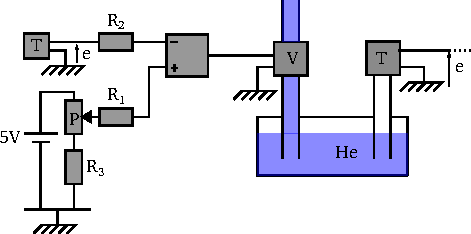
\includegraphics[width=0.8\linewidth]{circuit_10.pdf}
\end{figure}

Comment fonctionne ce montage ? Donnez la hauteur minimale $h_{min}$ et maximale $h_{max}$. Quel est le défaut de ce système ?

\subsection*{Seconde version}
On introduit une rétroaction sur l'AO avec une résistance.

\begin{figure}[!h]
\centering
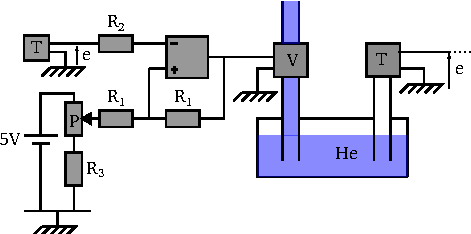
\includegraphics[width=0.8\linewidth]{circuit_11.pdf}
\end{figure}

Comment fonctionne ce nouveau montage ? Quel est son intérêt ? Donnez la hauteur minimale $h_{min}$ et maximale $h_{max}$.

\newpage

\section*{\textit{Correction : Remplissage d'un réservoir d'hélium}}

\subsection*{Première version}
\begin{itemize}
	\item[•] Pas de boucle de rétroaction : l'AO fonctionne forcément en régime saturé car la condition $u_+=u_-$ n'est jamais remplie. L'AO marche donc en comparateur et comme il est parfait $I_+=i_-=0$. Les résistances $R_1$ et $R_2$ sont inutiles.
	\item[•] Le potentiomètre fonctionne comme 2 résistances $(1-x)R_P$ et $xR_P$. Le potentiel (au niveau de la flèche) est pris entre ces 2 résistances. On a donc $u_+=\frac{xR_P+R_3}{R_P+R_3}U$, avec $U=5$V. La vanne s'ouvre lorsque $u_+>u_-$ cad pour :
	\begin{equation}
		u_+>u_-\Rightarrow\frac{xR_P+R_3}{R_P+R_3}U>\alpha h_{min}
	\end{equation}
	De même, la vanne se ferme lorsque :
	\begin{equation}
		u_+<	u_-\Rightarrow\frac{xR_P+R_3}{R_P+R_3}U<\alpha h_{max}
	\end{equation}
	On trouve que $h_{min}=h_{max}\in\left[ 0,2;1\right] $ pour x variant de 0 à 1.
	On a donc bien un système qui verse de l'hélium lorsque la hauteur descend en dessous de $h_{min}$ et s'arrête lorsque la hauteur atteint $h_{max}$. Le défaut est que $h_{min}=h_{max}$ : la vanne s'ouvre et se referme en permanence.
\end{itemize}

\subsection*{Seconde version}

\begin{itemize}
	\item[•] L'AO fonctionne toujours en régime saturé car la boucle de rétroaction est sur la borne +. $u_P$ est inchangé car les résistances $R_1$ sont très grandes devant les autres. On a donc $u_+=\frac{1}{2}u_s +\frac{1}{2}u_p$
	Si la vanne est initialement fermée, celle-ci s'ouvre lorsque le niveau atteint un niveau $h_{min}$ qui correspond à :
	\begin{equation}
		u_+=\frac{1}{2}V_{sat+} +\frac{1}{2}u_p=\alpha h_{min}
	\end{equation}
De même, si la vanne est initialement ouverte, celle-ci se ferme lorsque le niveau atteint un niveau $h_{max}$ qui correspond à :
	\begin{equation}
		u_+=\frac{1}{2}V_{sat-} +\frac{1}{2}u_p=\alpha h_{min}
	\end{equation}
	
	On a alors : $h_{min}=0,1$m et $h_{max}=1,1$m si $x=0$ et $h_{min}=0,5$m et $h_{max}=1,5$m si $x=1$. Le système ne s'ouvre et ferme plus en permanence.
\end{itemize}

\end{document}
